\appendix
\chapter{Anhang}
\section{Graph-Datenbanken - Grundlegende technologische Aspekte}
\section{Graph-Datenbanken und -Frameworks - Ausgewählte Systeme}
\begin{figure}[H]

    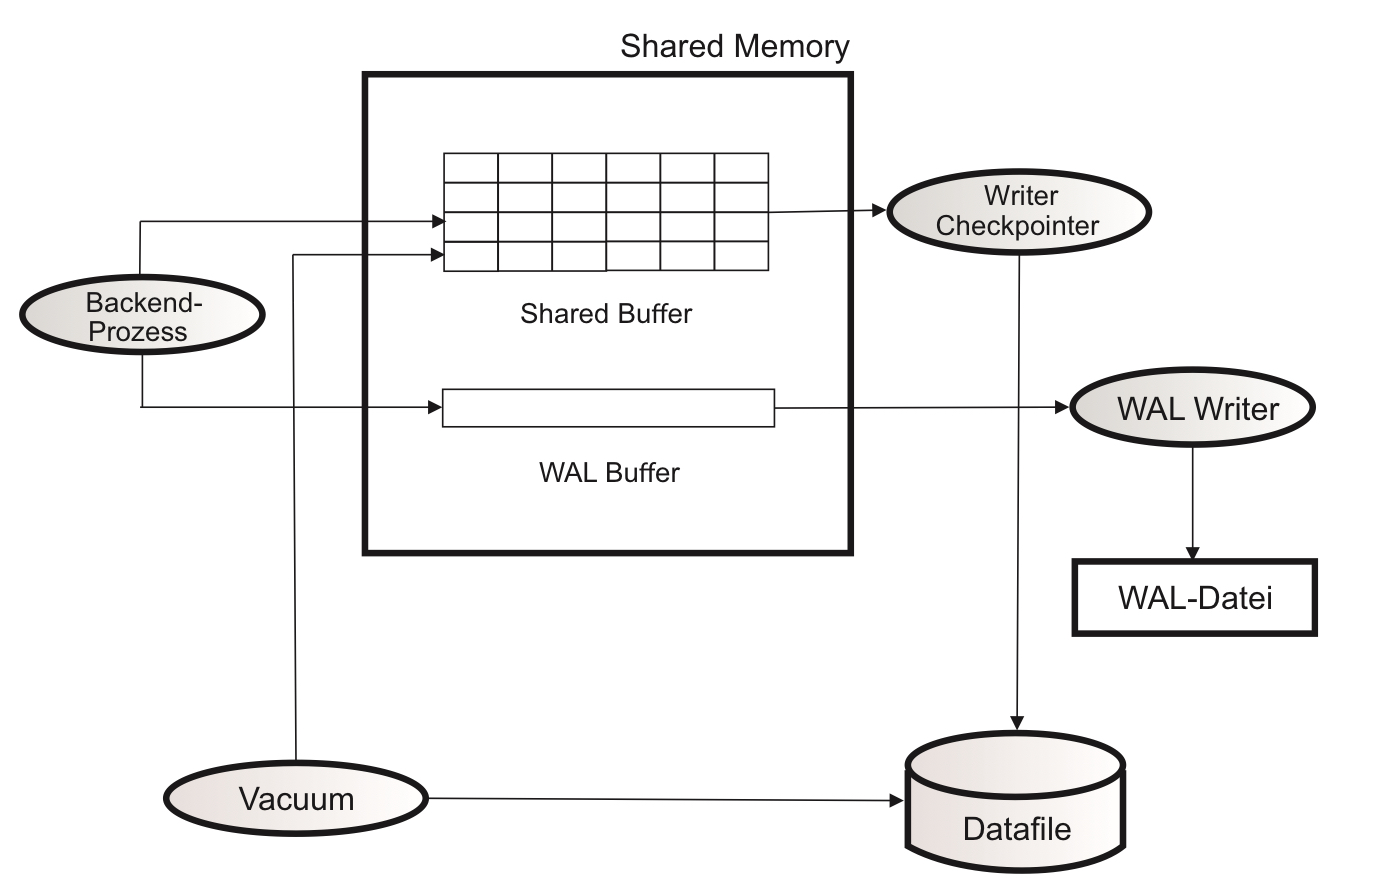
\includegraphics[width = \linewidth]{images/PostgresSQLArchitektur.jpg}
    \caption{Postgres Architektur}
    \label{2.Postgres Architektur.image}

\end{figure}
\section{Graph-Datenbanken im praktischen Einsatz: OLTP}
\lstsetsql
\begin{lstlisting}[language=SQL,caption=CSV Input,frame=single, label={2.copy.listing}]
    \copy Beitraege
    FROM './data/Beitraege.csv' DELIMITER ',' CSV HEADER;
\end{lstlisting}

\begin{lstlisting}[language=SQL,caption=Anlegen der Tabelle facebook-profiles,frame=single, label={2.facebookProfiles.listing}]
    create TABLE IF NOT EXISTS profiles_facebook(
    ID INTEGER PRIMARY KEY,
    first VARCHAR(50),
    last VARCHAR(50),
    gender GENDER,
    birth DATE,
    country VARCHAR(50)
    );
\end{lstlisting}

\begin{lstlisting}[language=SQL,caption=Anlegen der Tabelle facebook-relation,frame=single, label={2.relationFacebook.listing}]
    CREATE TABLE IF NOT EXISTS relation_facebook(
    src INTEGER REFERENCES profiles_facebook(ID),
    dst INTEGER REFERENCES profiles_facebook(ID),
    type VARCHAR(50),
    date DATE
    );
\end{lstlisting}

\begin{lstlisting}[language=SQL,caption=Hinzufügen von Fremdschlüsseln,frame=single, label={2.foreignKey.listing}]
    \copy profiles_facebook_tmp(first,last,gender,birth,country) FROM '/data/WS2018/facebook-profiles' DELIMITER ',' CSV HEADER;
    INSERT INTO profiles_facebook (ID, first, last, gender, birth, country)
    SELECT ID-1, first, last, gender, birth, country from profiles_facebook_tmp;
\end{lstlisting}

\begin{lstlisting}[language=SQL,caption=Erstellen von partitionierten Tabellen mit Index facebook,frame=single, label={2.parttableindexfacebook.listing}]
    CREATE TABLE IF NOT EXISTS relation_facebook_partitioned(
    src INTEGER REFERENCES profiles_facebook(ID),
    dst INTEGER REFERENCES profiles_facebook(ID),
    type VARCHAR(50),
    date DATE
    )PARTITION BY RANGE(src);

    CREATE INDEX fb_part_src ON relation_facebook_partitioned (src);
    CREATE INDEX fb_part_dst ON relation_facebook_partitioned (dst);

    CREATE TABLE relation_facebook_partitioned_0 PARTITION OF relation_facebook_partitioned
    FOR VALUES FROM (0) TO (23000);
    CREATE TABLE relation_facebook_partitioned_1 PARTITION OF relation_facebook_partitioned
    FOR VALUES FROM (23000) TO (46000);
    CREATE TABLE relation_facebook_partitioned_2 PARTITION OF relation_facebook_partitioned
    FOR VALUES FROM (46000) TO (69000);
    CREATE TABLE relation_facebook_partitioned_3 PARTITION OF relation_facebook_partitioned
    FOR VALUES FROM (69000) TO (92000);
\end{lstlisting}

\begin{lstlisting}[language=SQL,caption=Erstellen von Indexen auf relation Tabelle facebook,frame=single, label={2.indexfacebook.listing}]
    CREATE INDEX fb_dst ON relation_facebook_with_index (dst);
    CREATE INDEX fb_src ON relation_facebook_with_index (src);
\end{lstlisting}

\begin{lstlisting}[language=SQL,caption=Erstellen von partitionierten Tabellen mit Index youtube,frame=single, label={2.parttableindexyoutube.listing}]
    CREATE TABLE IF NOT EXISTS relation_youtube_partitioned(
    src INTEGER REFERENCES profiles_youtube(ID),
    dst INTEGER REFERENCES profiles_youtube(ID),
    type VARCHAR(50),
    date DATE
    )PARTITION BY RANGE(src);

    CREATE INDEX yt_part_src ON relation_youtube_partitioned (src);
    CREATE INDEX yt_part_dst ON relation_youtube_partitioned (dst);

    CREATE TABLE relation_youtube_partitioned_0 PARTITION OF relation_youtube_partitioned
    FOR VALUES FROM (0) TO (800000);
    CREATE TABLE relation_youtube_partitioned_1 PARTITION OF relation_youtube_partitioned
    FOR VALUES FROM (800001) TO (1600000);
    CREATE TABLE relation_youtube_partitioned_2 PARTITION OF relation_youtube_partitioned
    FOR VALUES FROM (1600001) TO (2400000);
    CREATE TABLE relation_youtube_partitioned_3 PARTITION OF relation_youtube_partitioned
    FOR VALUES FROM (2400001) TO (3200000);
\end{lstlisting}

\begin{lstlisting}[language=SQL,caption=Erstellen von Indexen auf relation Tabelle youtube,frame=single, label={2.indexyoutube.listing}]
    CREATE INDEX yt_dst ON relation_youtube_with_index (dst);
    CREATE INDEX yt_src ON relation_youtube_with_index (src);
\end{lstlisting}

\begin{lstlisting}[language=SQL,caption=Erstellen von partitionierten Tabellen mit Index livejournal,frame=single, label={2.parttableindexlivejournal.listing}]
    CREATE TABLE IF NOT EXISTS relation_livejournal_partitioned(
    src INTEGER REFERENCES profiles_livejournal(ID),
    dst INTEGER REFERENCES profiles_livejournal(ID),
    type VARCHAR(50),
    date DATE
    )PARTITION BY RANGE(src);

    CREATE INDEX lj_part_src ON relation_livejournal_partitioned (src);
    CREATE INDEX lj_part_dst ON relation_livejournal_partitioned (dst);

    CREATE TABLE relation_livejournal_partitioned_0 PARTITION OF relation_livejournal_partitioned
    FOR VALUES FROM (0) TO (10000000);
    CREATE TABLE relation_livejournal_partitioned_1 PARTITION OF relation_livejournal_partitioned
    FOR VALUES FROM (10000000) TO (20000000);
    CREATE TABLE relation_livejournal_partitioned_2 PARTITION OF relation_livejournal_partitioned
    FOR VALUES FROM (20000000) TO (30000000);
    CREATE TABLE relation_livejournal_partitioned_3 PARTITION OF relation_livejournal_partitioned
    FOR VALUES FROM (30000000) TO (40000000);
\end{lstlisting}

\begin{lstlisting}[language=SQL,caption=Erstellen von Indexen auf relation Tabelle livejournal,frame=single, label={2.indexlivejournal.listing}]
    CREATE INDEX lj_src ON relation_livejournal_with_index (src);
    CREATE INDEX lj_dst ON relation_livejournal_with_index (dst);
\end{lstlisting}

\begin{lstlisting}[language=SQL,caption=Erstellen von partitionierten Tabellen mit Index epinion,frame=single, label={2.parttableindexepinion.listing}]
    CREATE TABLE IF NOT EXISTS relation_epinions_partitioned(
    src INTEGER REFERENCES profiles_epinions(ID),
    dst INTEGER REFERENCES profiles_epinions(ID),
    type VARCHAR(50),
    date DATE
    )PARTITION BY RANGE(src);

    CREATE INDEX ep_part_src ON relation_epinions_partitioned (src);
    CREATE INDEX ep_part_dst ON relation_epinions_partitioned (dst);

    CREATE TABLE relation_epinions_partitioned_0 PARTITION OF relation_epinions_partitioned
    FOR VALUES FROM (0) TO (102000);
    CREATE TABLE relation_epinions_partitioned_1 PARTITION OF relation_epinions_partitioned
    FOR VALUES FROM (102000) TO (204000);
    CREATE TABLE relation_epinions_partitioned_2 PARTITION OF relation_epinions_partitioned
    FOR VALUES FROM (204000) TO (306000);
    CREATE TABLE relation_epinions_partitioned_3 PARTITION OF relation_epinions_partitioned
    FOR VALUES FROM (306000) TO (408000);
\end{lstlisting}

\begin{lstlisting}[language=SQL,caption=Erstellen von Indexen auf relation Tabelle epinion,frame=single, label={2.indexepinion.listing}]
    CREATE INDEX ep_dst ON relation_epinions_with_index (dst);
    CREATE INDEX ep_src ON relation_epinions_with_index (src);
\end{lstlisting}

\begin{lstlisting}[language=SQL,caption=Erstellen von partitionierten Tabellen mit wikivote epinion,frame=single, label={2.parttableindexwikivote.listing}]
    CREATE TABLE IF NOT EXISTS relation_wiki_vote_partitioned(
    src INTEGER REFERENCES profiles_wiki_vote(ID),
    dst INTEGER REFERENCES profiles_wiki_vote(ID),
    type VARCHAR(50),
    date DATE
    )PARTITION BY RANGE(src);

    CREATE INDEX wv_part_src ON relation_wiki_vote_partitioned (src);
    CREATE INDEX wv_part_dst ON relation_wiki_vote_partitioned (dst);

    CREATE TABLE relation_wiki_vote_partitioned_0 PARTITION OF relation_wiki_vote_partitioned
    FOR VALUES FROM (0) TO (30000);
    CREATE TABLE relation_wiki_vote_partitioned_1 PARTITION OF relation_wiki_vote_partitioned
    FOR VALUES FROM (30000) TO (60000);
    CREATE TABLE relation_wiki_vote_partitioned_2 PARTITION OF relation_wiki_vote_partitioned
    FOR VALUES FROM (60000) TO (90000);
    CREATE TABLE relation_wiki_vote_partitioned_3 PARTITION OF relation_wiki_vote_partitioned
    FOR VALUES FROM (90000) TO (120000);
\end{lstlisting}

\begin{lstlisting}[language=SQL,caption=Erstellen von Indexen auf relation Tabelle wikivote,frame=single, label={2.indexwikivote.listing}]
    CREATE INDEX wv_src ON relation_wiki_vote_with_index (src);
    CREATE INDEX wv_dst ON relation_wiki_vote_with_index (dst);
\end{lstlisting}

\begin{lstlisting}[language=SQL,caption=Erstellen der Indexe für die relation Tabelle facebook,frame=single, label={2.indexfacebook.listing}]
    CREATE INDEX fb_dst ON relation_facebook_with_index (dst);
    CREATE INDEX fb_src ON relation_facebook_with_index (src);
\end{lstlisting}

\begin{lstlisting}[language=SQL,caption = Verschachteltes SELECT Statement,frame=single,label={2.SELECT.listing} ]
    SELECT DISTINCT(dst) FROM team22.relation_facebook WHERE src IN(
    SELECT DISTINCT(dst) FROM team22.relation_facebook WHERE src IN(
    SELECT DISTINCT(dst)FROM team22.relation_facebook WHERE src IN(1)
    )
    )
\end{lstlisting}

\begin{lstlisting}[language=SQL,caption = SELECT SourceCodeGenerator ,frame=single, label={2.SelectSourceCodeGenerator.listing} ]
    CREATE OR REPLACE FUNCTION selectCascadingGenerator(iRecursionDepth integer, sTable text, startingNode integer ) RETURNS SETOF integer AS $$
    Declare
    intermDst_ integer[];
    --  iCount integer;
    tStatement text;
    tConcatenateStatement text;
    BEGIN
    tConcatenateStatement := 'SELECT DISTINCT(dst) FROM ' || sTable || ' WHERE src IN(';
    tStatement := 'SELECT DISTINCT(dst) FROM ' || sTable || ' WHERE src IN('||startingNode||')';
    --   iCount = 0;
    if iRecursionDepth = 0 THEN
    return query EXECUTE tStatement;
    RETURN;
    end if;
    WHILE iRecursionDepth > 1 LOOP
    tStatement := tConcatenateStatement || tStatement ||')';
    iRecursionDepth = iRecursionDepth - 1;
    end loop;
    raise notice 'Execute String %', tStatement;
    return query EXECUTE tStatement;
    END;
    $$ LANGUAGE plpgsql;
\end{lstlisting}

\begin{lstlisting}[language=SQL,caption = Rekursiver JOIN,frame=single, label={2.JOIN.listing} ]
    SELECT DISTINCT(rf3.dst)
    FROM public.relation_facebook rf1,
    public.relation_facebook rf2,
    public.relation_facebook rf3
    WHERE rf2.src = rf1.dst
    AND rf3.src = rf2.dst
    AND rf1.src = 765;
\end{lstlisting}

\begin{lstlisting}[language=SQL,caption = innerJoinSourceCodeGenerator,frame=single, label={2.INNERJOINGENERATOR.listing} ]
    CREATE OR REPLACE FUNCTION innerJoinGenerator(iRecursionDepth integer, sTable text, iStart integer) RETURNS SETOF integer AS $$
    Declare
    intermDst_ integer[];
    iCount integer;
    tStatement text;
    tSelectStatement text;
    tConcatenateStatement text;
    tAlternativeStatement text;
    tWhereStatement text;
    tFinalStatement text;
    tSetOffMergeJoin text;
    BEGIN
    tSetOffMergeJoin = 'set enable_mergejoin=on;';
    iCount = 0;
    tSelectStatement = '';
    tWhereStatement = '';
    tConcatenateStatement := 'SELECT DISTINCT(dst) FROM ' || sTable || ' WHERE src IN(';
    tStatement := sTable || ' rf';
    tAlternativeStatement = sTable || ' rf';
    --   iCount = 0;
    if iRecursionDepth = 0 THEN
    raise notice 'Rekursivtiefe von 0 nicht m\"oglich';
    RETURN ;
    end if;
    if iRecursionDepth = 1 THEN
    tConcatenateStatement = tConcatenateStatement || iStart || ')';
    raise notice 'STATEMENT: %', tConcatenateStatement;
    return query EXECUTE tConcatenateStatement;
    RETURN;
    end if;
    WHILE iCount < iRecursionDepth LOOP
    if iCount = iRecursionDepth - 1 then
    tSelectStatement := tSelectStatement || tStatement  || iCount || ' ';
    else
    tSelectStatement := tSelectStatement || tStatement  || iCount || ', ';
    end if;
    if iCount != 0 then
    if iCount = iRecursionDepth - 1 then
    tWhereStatement := tWhereStatement || 'rf' || iCount || '.src = rf' || iCount - 1 || '.dst ';
    else
    tWhereStatement := tWhereStatement || 'rf' || iCount || '.src = rf' || iCount - 1 || '.dst AND ';
    end if;
    else
    tWhereStatement := 'rf' || iCount || '.src = '|| iStart || ' AND ' ;
    end if;
    iCount = iCount + 1;
    end loop;
    tWhereStatement := 'WHERE ' || tWhereStatement;
    tSelectStatement := 'FROM ' || tSelectStatement;
    tFinalStatement = 'SELECT DISTINCT(rf'||iRecursionDepth - 1 || '.dst) ' || tSelectStatement || tWhereStatement;
    raise notice 'FROM Statement: %', tSelectStatement;
    raise notice 'Where Statement: %', tWhereStatement;
    raise notice 'Finale Statement: %', tFinalStatement;
    EXECUTE tSetOffMergeJoin;
    return query EXECUTE tFinalStatement;
    END;
    $$ LANGUAGE plpgsql;
\end{lstlisting}

\newpage
\begin{lstlisting}[language=SQL,caption = Selbstgeschriebenes Stored Procedure,frame=single, label={2.recursiveFunction.listing} ]
    CREATE OR REPLACE FUNCTION recursivesearch(tInput integer[], iRecursionDepth integer, sTable text) RETURNS SETOF integer AS $$
    Declare
    intermDst_ integer[];
    iCount integer;
    BEGIN
    --iRecursionDepth = iRecursionDepth + 1;
    CREATE TEMPORARY TABLE intermDst AS SELECT * FROM unnest(tInput);
    EXECUTE 'CREATE TEMPORARY TABLE intermDst1 AS SELECT DISTINCT(dst) FROM ' || sTable || ' WHERE src IN (SELECT * FROM intermDst)';
    -- Does not return from function!
    return query SELECT * FROM intermDst1;
    -- Does not return from function!
    intermDst_ := ARRAY(SELECT * FROM intermDst1);
    raise notice 'timestamp: %', clock_timestamp();
    SELECT count(*) INTO iCount FROM intermDst;
    raise notice 'Count Table: %', iCount;
    DROP TABLE intermDst;
    DROP TABLE intermDst1;
    -- As recursion depth is 5
    if iRecursionDepth > 1 THEN
    return query SELECT * FROM recursivesearch(intermDst_, iRecursionDepth - 1, sTable);
    ELSE
    RETURN;
    END IF;
    END;
    $$ LANGUAGE plpgsql;
\end{lstlisting}

\begin{lstlisting}[language=SQL,caption = SQL Standard Generisch,frame=single, label={2.StandardSQLGenerisch.listing} ]
    CREATE OR REPLACE FUNCTION selectWithUnionSourceCodeGenerator_withDepth(sTable text, startingNode integer, depth integer ) RETURNS SETOF integer AS $$
    Declare
    intermDst_ integer[];
    tStatement text;
    tSelectStatement text;
    tWithStatement text;
    tUnionStatement text;
    tWithStatementClose text;
    BEGIN
    tWithStatement := 'WITH RECURSIVE graphtraverse(src, dst, lvl) AS(';
    tSelectStatement := 'SELECT src ,dst, 1 as lvl FROM ' || sTable || ' WHERE src ='||startingNode;
    tUnionStatement := ' UNION SELECT p1.src,p1.dst,p.lvl+1 as lvl FROM graphtraverse p, ' || sTable || ' p1 WHERE p1.src IN ( p.dst ) and lvl<'||depth;
    tWithStatementClose := ') SELECT DISTINCT(dst) FROM graphtraverse';
    tStatement := tWithStatement || tSelectStatement || tUnionStatement || tWithStatementClose;
    raise notice 'Execute String %', tStatement;
    return query EXECUTE tStatement;
    END;
    $$ LANGUAGE plpgsql;
\end{lstlisting}

\begin{lstlisting}[language=SQL,caption = SQL Standard,frame=single, label={2.StandardSQL.listing} ]
    WITH RECURSIVE graphtraverse(src, dst, lvl) AS(
    SELECT src ,dst, 1 as lvl FROM public.relation_facebook WHERE src =765
    UNION
    SELECT p1.src,p1.dst,p.lvl+1 as lvl FROM graphtraverse p, relation_facebook p1 WHERE p1.src IN ( p.dst ) and lvl<5
    ) SELECT DISTINCT(dst) FROM graphtraverse order by dst;
\end{lstlisting}

\begin{lstlisting}[language=SQL,caption = Ausführungsplan Standard SQL,frame=single, label={2.AusführungsplanCTEFacebook.listing} ]
    Sort  (cost=15300.01..15300.51 rows=200 width=4) (actual time=17.613..17.622 rows=321 loops=1)
    Sort Key: graphtraverse.dst
    Sort Method: quicksort  Memory: 40kB
    CTE graphtraverse
    ->  Recursive Union  (cost=0.29..14814.87 rows=21133 width=12) (actual time=0.016..15.903 rows=6056 loops=1)
    ->  Index Scan using indexsrc on relation_facebook  (cost=0.29..44.00 rows=23 width=12) (actual time=0.015..0.020 rows=27 loops=1)
    Index Cond: (src = 765)
    ->  Nested Loop  (cost=0.29..1434.82 rows=2111 width=12) (actual time=0.019..2.130 rows=8173 loops=5)
    ->  WorkTable Scan on graphtraverse p  (cost=0.00..5.17 rows=77 width=8) (actual time=0.017..0.069 rows=729 loops=5)
    Filter: (lvl < 5)
    Rows Removed by Filter: 482
    ->  Index Scan using indexsrc on relation_facebook p1  (cost=0.29..18.23 rows=27 width=8) (actual time=0.001..0.002 rows=11 loops=3645)
    Index Cond: (src = p.dst)
    ->  HashAggregate  (cost=475.49..477.49 rows=200 width=4) (actual time=17.548..17.571 rows=321 loops=1)
    Group Key: graphtraverse.dst
    ->  CTE Scan on graphtraverse  (cost=0.00..422.66 rows=21133 width=4) (actual time=0.017..16.771 rows=6056 loops=1)
    Planning Time: 0.105 ms
    Execution Time: 17.813 ms
\end{lstlisting}

\begin{lstlisting}[language=SQL,caption = Ausführungsplan verschachteltes SELECT,frame=single, label={2.AusführungsplanCascadeSELECT.listing} ]
    HashAggregate  (cost=6623.97..6659.95 rows=3598 width=4) (actual time=27.019..27.049 rows=317 loops=1)
    Group Key: relation_facebook.dst
    ->  Hash Join  (cost=4727.16..6403.39 rows=88234 width=4) (actual time=20.593..26.743 rows=2411 loops=1)
    Hash Cond: (relation_facebook.src = relation_facebook_1.dst)
    ->  Seq Scan on relation_facebook  (cost=0.00..1444.34 rows=88234 width=8) (actual time=0.008..3.889 rows=88234 loops=1)
    ->  Hash  (cost=4682.18..4682.18 rows=3598 width=4) (actual time=18.021..18.021 rows=195 loops=1)
    Buckets: 4096  Batches: 1  Memory Usage: 39kB
    ->  HashAggregate  (cost=4610.22..4646.20 rows=3598 width=4) (actual time=17.976..18.000 rows=195 loops=1)
    Group Key: relation_facebook_1.dst
    ->  Hash Join  (cost=2713.40..4389.64 rows=88234 width=4) (actual time=11.821..17.797 rows=1709 loops=1)
    Hash Cond: (relation_facebook_1.src = relation_facebook_2.dst)
    ->  Seq Scan on relation_facebook relation_facebook_1  (cost=0.00..1444.34 rows=88234 width=8) (actual time=0.002..3.916 rows=88234 loops=1)
    ->  Hash  (cost=2668.43..2668.43 rows=3598 width=4) (actual time=9.177..9.177 rows=144 loops=1)
    Buckets: 4096  Batches: 1  Memory Usage: 38kB
    ->  HashAggregate  (cost=2596.47..2632.45 rows=3598 width=4) (actual time=9.140..9.161 rows=144 loops=1)
    Group Key: relation_facebook_2.dst
    ->  Hash Join  (cost=876.96..2553.22 rows=17301 width=4) (actual time=2.942..9.020 rows=1280 loops=1)
    Hash Cond: (relation_facebook_2.src = relation_facebook_3.dst)
    ->  Seq Scan on relation_facebook relation_facebook_2  (cost=0.00..1444.34 rows=88234 width=8) (actual time=0.002..4.163 rows=88234 loops=1)
    ->  Hash  (cost=869.07..869.07 rows=631 width=4) (actual time=0.276..0.276 rows=88 loops=1)
    Buckets: 1024  Batches: 1  Memory Usage: 12kB
    ->  HashAggregate  (cost=856.45..862.76 rows=631 width=4) (actual time=0.259..0.268 rows=88 loops=1)
    Group Key: relation_facebook_3.dst
    ->  Nested Loop  (cost=44.35..854.88 rows=631 width=4) (actual time=0.022..0.199 rows=629 loops=1)
    ->  HashAggregate  (cost=44.05..44.28 rows=23 width=4) (actual time=0.018..0.021 rows=27 loops=1)
    Group Key: relation_facebook_4.dst
    ->  Index Scan using indexsrc on relation_facebook relation_facebook_4  (cost=0.29..44.00 rows=23 width=4) (actual time=0.009..0.012 rows=27 loops=1)
    Index Cond: (src = 765)
    ->  Index Scan using indexsrc on relation_facebook relation_facebook_3  (cost=0.29..34.96 rows=27 width=8) (actual time=0.002..0.005 rows=23 loops=27)
    Index Cond: (src = relation_facebook_4.dst)
    Planning Time: 0.170 ms
    Execution Time: 27.113 ms


\end{lstlisting}

\begin{lstlisting}[language=SQL,caption = Ausführungsplan INNER JOIN,frame=single, label={2.AusführungsplanINNERJOIN.listing} ]
    HashAggregate  (cost=172324.88..172360.86 rows=3598 width=4) (actual time=156.786..156.823 rows=317 loops=1)
    Group Key: rf5.dst
    Buffers: shared hit=2654
    ->  Merge Join  (cost=38989.73..153806.87 rows=7407207 width=4) (actual time=33.728..105.213 rows=572149 loops=1)
    Merge Cond: (rf5.src = rf4.dst)
    Buffers: shared hit=2654
    ->  Index Scan using indexsrc on relation_facebook rf5  (cost=0.29..3539.96 rows=88234 width=8) (actual time=0.004..3.466 rows=33654 loops=1)
    Buffers: shared hit=331
    ->  Sort  (cost=38972.52..39749.91 rows=310956 width=4) (actual time=30.171..50.861 rows=579169 loops=1)
    Sort Key: rf4.dst
    Sort Method: quicksort  Memory: 6709kB
    Buffers: shared hit=2323
    ->  Merge Join  (cost=2353.66..10603.46 rows=310956 width=4) (actual time=9.093..21.946 rows=77587 loops=1)
    Merge Cond: (rf3.dst = rf4.src)
    Buffers: shared hit=2323
    ->  Sort  (cost=2333.95..2366.58 rows=13054 width=4) (actual time=3.176..3.593 rows=8177 loops=1)
    Sort Key: rf3.dst
    Sort Method: quicksort  Memory: 576kB
    Buffers: shared hit=1993
    ->  Nested Loop  (cost=0.88..1441.56 rows=13054 width=4) (actual time=0.012..2.289 rows=8177 loops=1)
    Buffers: shared hit=1993
    ->  Nested Loop  (cost=0.58..854.36 rows=548 width=4) (actual time=0.009..0.156 rows=629 loops=1)
    Buffers: shared hit=89
    ->  Index Scan using indexsrc on relation_facebook rf1  (cost=0.29..44.00 rows=23 width=4) (actual time=0.004..0.008 rows=27 loops=1)
    Index Cond: (src = 765)
    Buffers: shared hit=3
    ->  Index Scan using indexsrc on relation_facebook rf2  (cost=0.29..34.96 rows=27 width=8) (actual time=0.001..0.003 rows=23 loops=27)
    Index Cond: (src = rf1.dst)
    Buffers: shared hit=86
    ->  Index Scan using indexsrc on relation_facebook rf3  (cost=0.29..0.80 rows=27 width=8) (actual time=0.001..0.002 rows=13 loops=629)
    Index Cond: (src = rf2.dst)
    Buffers: shared hit=1904
    ->  Materialize  (cost=0.29..3760.54 rows=88234 width=8) (actual time=0.004..8.301 rows=109531 loops=1)
    Buffers: shared hit=330
    ->  Index Scan using indexsrc on relation_facebook rf4  (cost=0.29..3539.96 rows=88234 width=8) (actual time=0.003..3.863 rows=33653 loops=1)
    Buffers: shared hit=330
    Planning Time: 0.627 ms
    Execution Time: 157.021 ms

\end{lstlisting}

\section{Graph-Datenbanken im praktischen Einsatz: OLAP}
%\chapter{Anhang}
%Appendix